\documentclass{standalone}
\usepackage{tikz}

\begin{document}
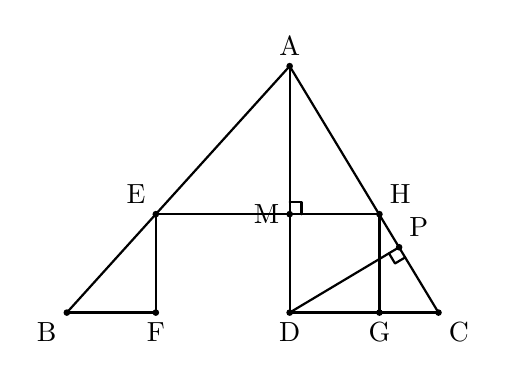
\begin{tikzpicture}[line cap=round, line join=round, thick]

  % 关键点坐标（单位：cm）
  \coordinate (A) at (3.50,3.13);
  \coordinate (B) at (0.67,0);
  \coordinate (C) at (5.39,0);
  \coordinate (D) at (3.50,0);
  \coordinate (F) at (1.80,0);
  \coordinate (G) at (4.64,0);
  \coordinate (E) at (1.80,1.25);
  \coordinate (H) at (4.64,1.25);
  \coordinate (M) at (3.50,1.25);
  % 垂足 P：D 到直线 CH 的垂足
  \coordinate (P) at (4.89,0.83);

  % 三角形两腰
  \draw (A) -- (B);
  \draw (A) -- (C);

  % 底边 BC（去掉线段 DF 的笔画）
  \draw (B) -- (F);
  \draw (D) -- (G);
  \draw (G) -- (C);

  % 矩形 EFGH 的边
  \draw (E) -- (H);
  \draw (E) -- (F);
  \draw (H) -- (G);

  % 高线 AD
  \draw (A) -- (D);

  % 直角标记（AD 与 EH 的交点 M 处）
  \draw (3.50,1.40) -- (3.65,1.40) -- (3.65,1.25);

  % 垂线 DP
  \draw (D) -- (P);

  % 直角标记（P 处）
  \draw (4.967,0.701) -- (4.838,0.624) -- (4.761,0.753);

  % 点标记（保留 D、F 及其标签）
  \fill (A) circle (1.2pt) node[above] {A};
  \fill (B) circle (1.2pt) node[below left] {B};
  \fill (C) circle (1.2pt) node[below right] {C};
  \fill (D) circle (1.2pt) node[below] {D};
  \fill (F) circle (1.2pt) node[below] {F};
  \fill (G) circle (1.2pt) node[below] {G};
  \fill (E) circle (1.2pt) node[above left] {E};
  \fill (H) circle (1.2pt) node[above right] {H};
  \fill (M) circle (1.2pt) node[left] {M};
  \fill (P) circle (1.2pt) node[above right] {P};

\end{tikzpicture}
\end{document}
